O SUM, para atender as necessidades do projeto, estará localizado nos terraços dos três prédios do campus, assim poderá abranger uma maior área de vigilância do estacionamento da FGA trazendo assim uma maior segurança e comodidade aos alunos e professores.

O balão cativo ZP (Zero Pressão) necessitará de três pontos de fixação. Destes três, dois pontos estarão fixos no topo do respectivos prédios e o terceiro ponto será fixado em um poste de sustentação que terá a altura do prédio cerca de 10 metros de altura e estará distante 5 metros perpendicularmente ao mesmo.

O gás do balão sairá do envelope, na pior das possibilidades, a uma taxa de 7.9\% por dia, desta forma deve-se reabastecer o balão com hélio semanalmente. Os cálculos indicam que ao final de sete dias ainda restará 63.5 $m^{3}$. Para a reposição do gás, a manutenção terá de ser feita semanalmente em solo. Considerando que estas serão realizadas nos terraços dos prédios (UED, UAC e RU), haverá a necessidade de descer o balão. Para isso, serão instalados em dois pontos fixos dos prédios motores elétricos com capacidade de carga de 3863Kg e potência de 3800W capazes de puxar o balão e manter a altitude fixa. Nos motores, assim como no ponto de fixação fora do prédio, será utilizado o cabo de aço Alma de Fibra, que foi escolhido por ser mais leve que os cabos de aço comuns e possuir boa propriedades mecânicas.

Na figura \ref{img: Protótipo do Sum no Catia} está o protótipo do SUM. Nota-se que há uma fita de carga que passa no equador do envelope que segura a payload. A figura \ref{img: Protótipo da payload do Sum no Catia}  (a)  mostra como a payload deve ser amarrada ao balão. A figura \ref{img: Detalhe do trilho da payload} (b) mostra o detalhe do trilho na parte superior da payload, com esse trilho a payload pode se mover sem que haja perda no foco da imagem.
\begin{figure}[htp]
	\centering
	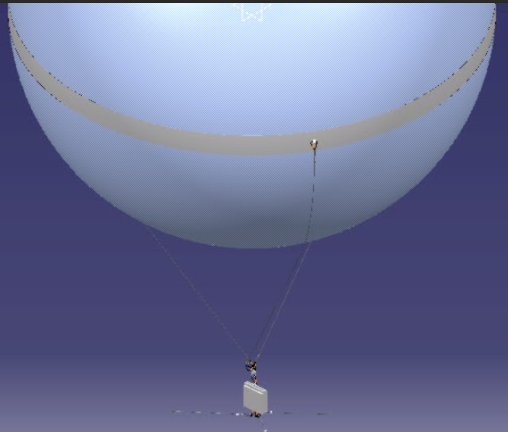
\includegraphics[scale=0.50]{figuras/catiadobalao}
	\caption{Protótipo do Sum no Catia}
	\label{img: Protótipo do Sum no Catia}
\end{figure}

\begin{figure}[htp]
	\centering
	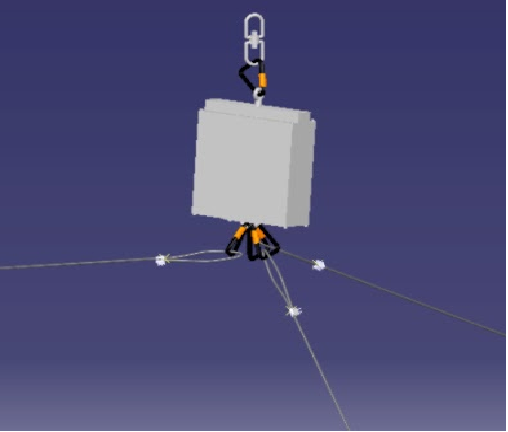
\includegraphics[scale=0.50]{figuras/catiadopayload}
	\caption{Protótipo da payload do Sum no Catia}
	\label{img: Protótipo da payload do Sum no Catia}
	\end{figure}

\begin{figure}[htp]
	\centering
	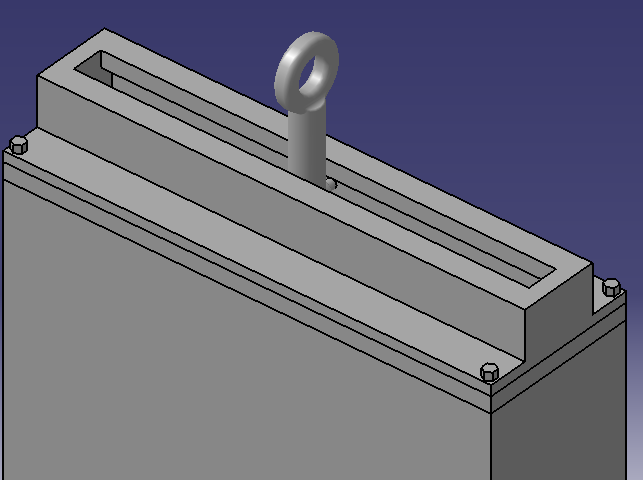
\includegraphics[scale=0.50]{figuras/catiadafixacao}
	\caption{Detalhe do trilho da payload}
	\label{img: Detalhe do trilho da payload}
\end{figure}

A inclusão dos trilhos e do sistema de estabilização fez-se necessário para manter a estabilidade da câmera, visando a qualidade na obtenção das imagens e tornando o sistema capaz de observar o estacionamento.

Para a melhor visualização do funcionamento integrado do SUM, apresenta-se uma situação hipotética de atividade suspeita.

Supondo que em uma das áreas de monitoramento definidas pela figura \ref{img: Mapa do Campus com as posições dos balões}, um indivíduo, numa distância horizontal de, aproximadamente, 5 metros do balão, encoste no veículo e não saia no mesmo durante 5 minutos,ou fique parado perto do carro a uma distancia de 2 metros sem sair no veiculo, será emitido um pequeno sinal de alerta na estação de solo e caso permaneça na mesma atitude por mais um minuto será emitido um sinal no monitor central da estação onde o operador irá averiguar a situação, e as câmeras passarão a filmar em vez de só transmitir.

\begin{figure}[htp]
\centering
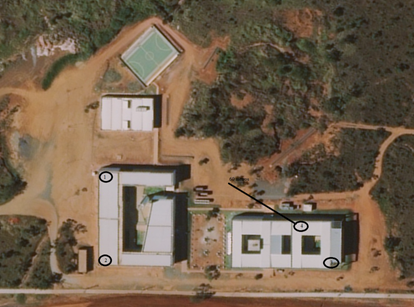
\includegraphics[scale=0.80]{figuras/campus}
\caption{Mapa do Campus com as posições dos balões}
\label{img: Mapa do Campus com as posições dos balões}
\end{figure}

O operador, que ficará na estação de solo, já tendo recebido o treinamento necessário para identificação das situações padrões de furto, (poderá aproximar a imagem, pois as câmeras Waveshare OV5647 Night Vision, definidas para serem acopladas à payload, possuem distância focal de 3.29 mm, com resolução de 5 Mega Pixels/ 1080p. O operador irá ver se a situação é realmente perigosa e caso sera necessário irá acionar  via rádio a segurança do campus para que algum outro segurança possa fazer a vistoria do local e caso seja necessário informara a policia.

A eletrônica embarcada, no processamento de imagens e transmissão de dados, realizará os seguintes processos: as imagens captadas pela câmera serão direcionadas para o Raspberry PI, através do seu conector específico para câmera. Este  conterá um algoritmo que realizará a compressão dos vídeos enviados, no padrão H264, um padrão de codificação de vídeo que utiliza um quadro de referência para comparação e codifica apenas os pixels que foram modificados.Após realizar esse processo de compressão, o Raspberry que estará conectado ao Arduino, receberá os dados dos sensores e a interpretação feita pelo algoritmo implementado no microcontrolador. Caso a interpretação do algoritmo informe determinada anomalia no sistema e exija que esse seja estabilizado, o Raspberry comunicará ao Galileo, via comunicação serial, que realize a estabilização do sistema.Com as imagens e os dados dos sensores obtidos, o Raspberry transmitirá essa informações em tempo real para o balão mais próximo da central, a comunicação entre eles será sem fio, montando uma rede intranet. O balão, que estará recebendo essas informações, transmitirá para a central através de um cabo de ethernet e o computador que recebe realizará todo o procedimento desejado com as imagens.

Com estas imagens e os dados dos sensores transmitidos, será realizado o reconhecimento da situação em questão e será verificado o funcionamento do sistema. A estação de solo possuirá um conjunto de monitores e um monitor central. Após a transmissão das informações, serão emitidos alertas no monitor central, onde o operador irá averiguar a situação e, caso seja necessário, informar a segurança do campus. A segurança do campus irá até o local e verificará a situação, tendo como responsabilidade informar a polícia, de acordo com o ocorrido.
